\section{Forecasting}
Two framings use the \texttt{last\_updated} time axis.
\begin{itemize}
  \item \textbf{City panel, next-day forecast}: one global model learns from all 197 capitals at once.
  \item \textbf{Global mean series, 60-day multi-step forecast}: the worldwide trend is projected forward.
\end{itemize}
Every model is a nested MLflow run with its parameters, validation and test metrics, a residual plot, the
model artefact and an input signature. Each one is also registered in the MLflow Model Registry
(\texttt{weather-temp-<model>}).

\paragraph{Metrics.} MAE, RMSE, sMAPE, $R^2$, and the share of forecasts within 2\,\textdegree C.
MAPE is computed only where $|y|\ge1$\,\textdegree C, because it explodes near 0\,\textdegree C. We also
report \emph{skill}, the RMSE reduction relative to persistence (tomorrow = today).

\subsection{City panel: single models and ensembles}
Four learners are compared against persistence:
\begin{itemize}
  \item ridge regression on the train-fitted standardisation;
  \item random forest;
  \item XGBoost and LightGBM, both with early stopping on the validation window.
\end{itemize}
Three ensembles are built from validation-window predictions only:
\begin{itemize}
  \item a simple mean;
  \item an inverse-validation-RMSE weighted mean;
  \item \textbf{stacking} with non-negative least squares. Its weights are XGBoost 0.49, LightGBM 0.26,
        Ridge 0.24 and random forest 0.01.
\end{itemize}
The stacked ensemble is logged as an MLflow \texttt{pyfunc} model (\texttt{weather-temp-ensemble}). The
pipeline checks that the served model reproduces the offline predictions.

\tbl{model_comparison.tex}

All learned models beat persistence. The ensembles beat every single model, and stacking is best:
test RMSE 1.838\,\textdegree C, MAE 1.21\,\textdegree C, $R^2=0.929$, 81\,\% of forecasts within 2\,\textdegree C,
and 12.2\,\% skill. Ridge receives a meaningful weight despite being the weakest member because its errors
are the least correlated with the tree models'. The gains look modest because day-to-day weather from a single
daily snapshot is noisy; the hardest regions are mid-latitude Europe and Asia, where synoptic systems pass
through (Figure~\ref{fig:rmsecont}).

\begin{figure}[H]\centering
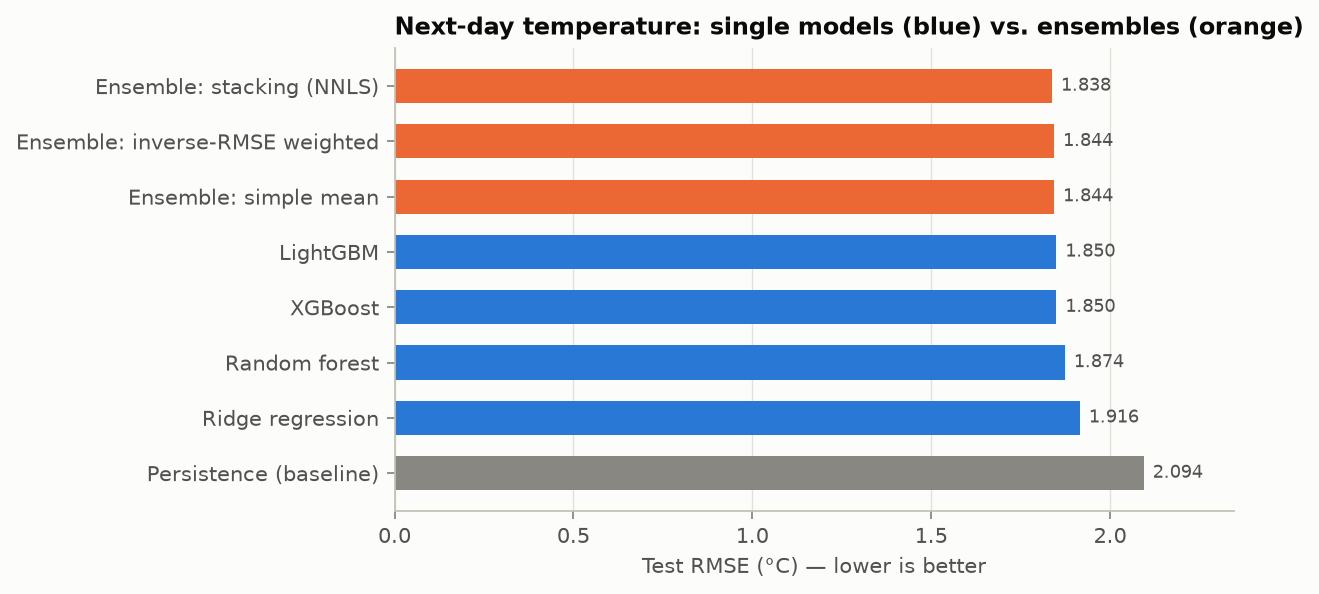
\includegraphics[width=0.85\linewidth]{forecast_panel/model_comparison_rmse.png}
\caption{Test RMSE of single models (blue) and ensembles (orange).}
\end{figure}
\begin{figure}[H]\centering
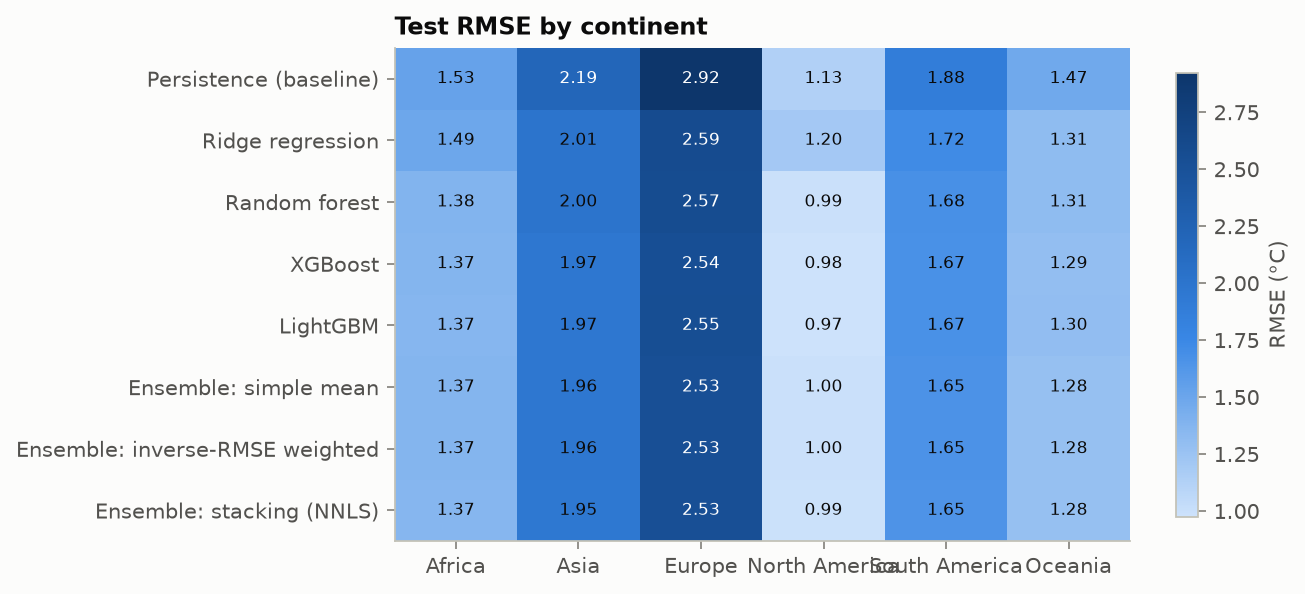
\includegraphics[width=0.85\linewidth]{forecast_panel/rmse_by_continent.png}
\caption{Test RMSE by continent.}\label{fig:rmsecont}
\end{figure}
\begin{figure}[H]\centering
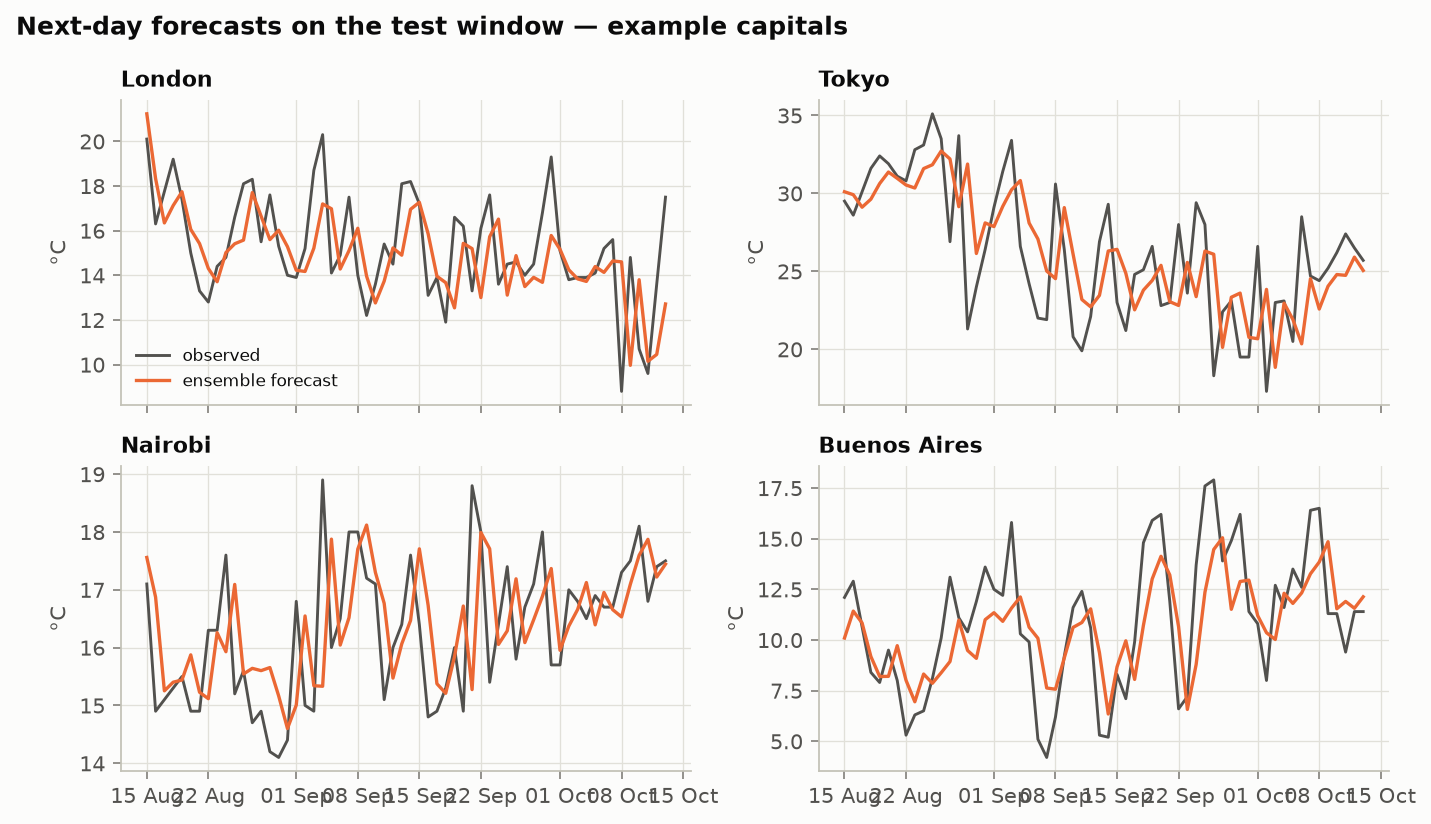
\includegraphics[width=0.9\linewidth]{forecast_panel/city_forecasts.png}
\caption{Stacked-ensemble next-day forecasts against observations for four example capitals.}
\end{figure}
\begin{figure}[H]\centering
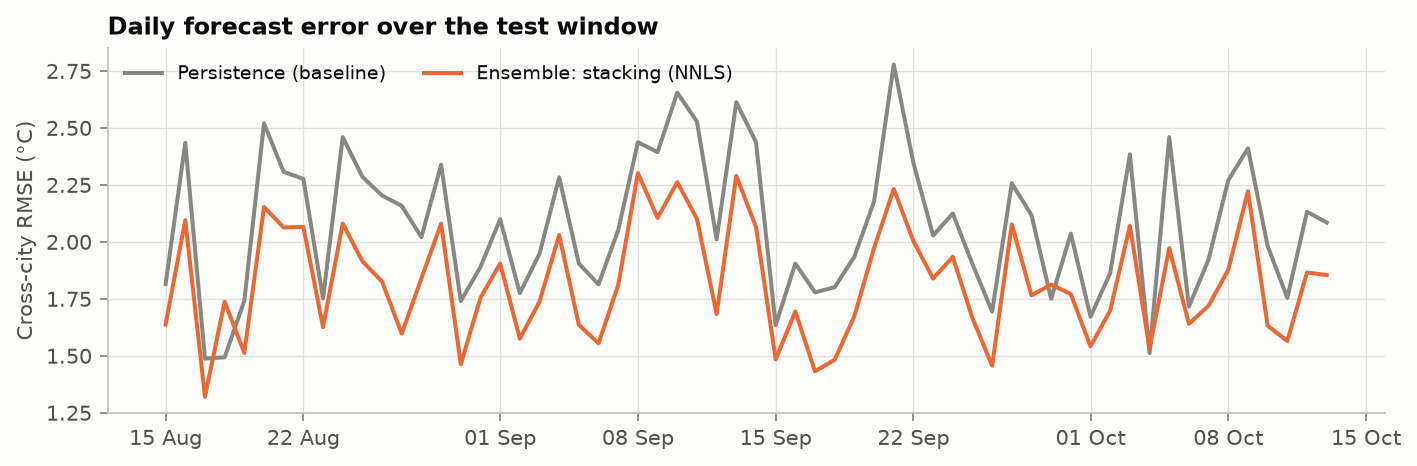
\includegraphics[width=0.9\linewidth]{forecast_panel/daily_error_test.png}
\caption{Cross-city RMSE per day over the test window.}
\end{figure}

\subsection{Global mean series: multi-step trend forecasting}
Each model is fitted on everything before the test window and forecasts all 60 test days in one shot:
\begin{itemize}
  \item naive and seasonal-naive (value 365 days earlier) baselines;
  \item damped Holt--Winters with a 365-day season;
  \item harmonic regression (trend, four annual harmonics, observation-hour harmonics);
  \item regression with ARIMA(1,0,1) errors on the same design (\texttt{sarimax\_fourier});
  \item their mean ensemble.
\end{itemize}
The snapshot hour of future days is unknown, so it is held at its last 30-day average.

\tbl{global_model_comparison.tex}

Harmonic regression and SARIMAX reach about 0.35\,\textdegree C RMSE over a 60-day horizon, four times
better than seasonal-naive. The ensemble is marginally best. Including the observation-hour terms cuts the
SARIMAX error from 0.62 to 0.37\,\textdegree C, which confirms that the confounder matters for forecasting
as well as for trend estimation. Refitted on all data, the best interval-producing model projects the next
90 days with a 95\,\% prediction interval (Figure~\ref{fig:future}).

\begin{figure}[H]\centering
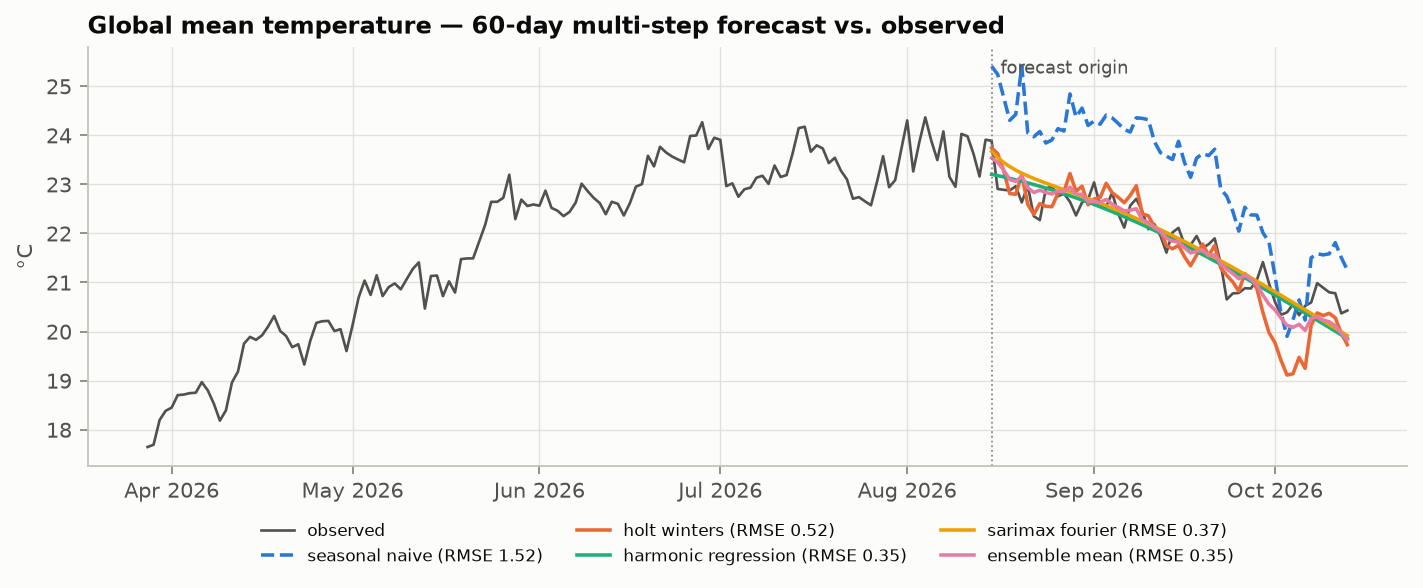
\includegraphics[width=0.9\linewidth]{forecast_global/global_multistep_forecast.png}
\caption{60-day multi-step forecasts of the global mean temperature.}
\end{figure}
\begin{figure}[H]\centering
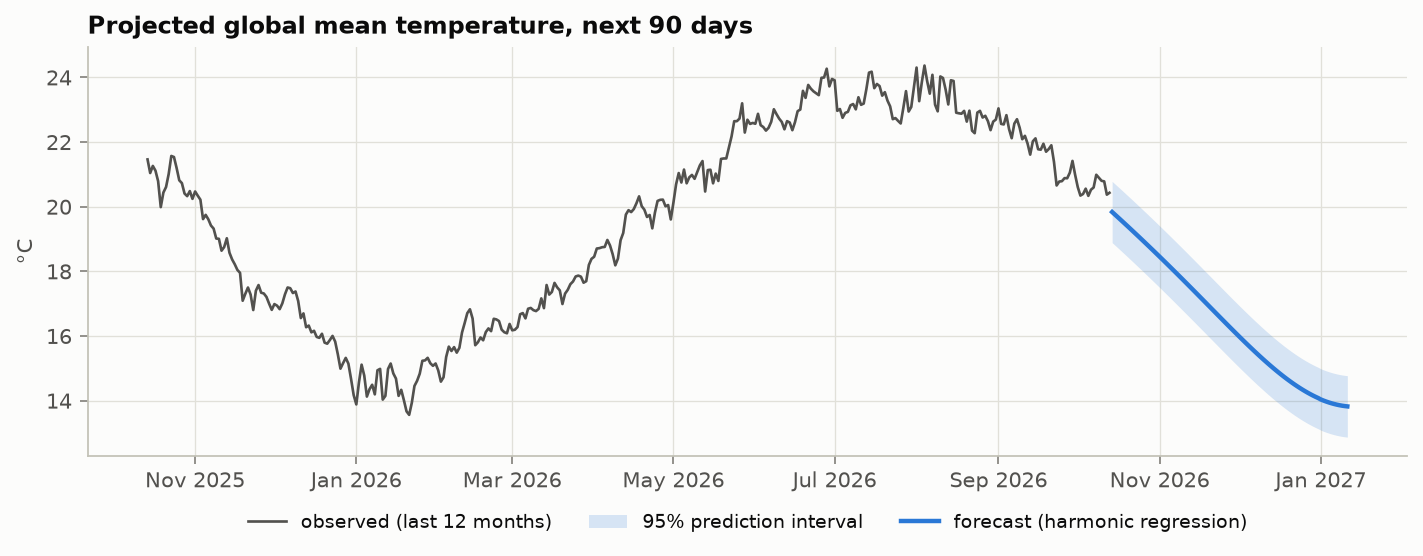
\includegraphics[width=0.9\linewidth]{forecast_global/global_future_forecast.png}
\caption{Projected global mean temperature for the next 90 days.}\label{fig:future}
\end{figure}
